\documentclass[10pt]{article}
\usepackage[polish]{babel}
\usepackage[utf8]{inputenc}
\usepackage[T1]{fontenc}
\usepackage{graphicx}
\usepackage[export]{adjustbox}
\graphicspath{ {./images/} }
\usepackage{amsmath}
\usepackage{amsfonts}
\usepackage{amssymb}
\usepackage[version=4]{mhchem}
\usepackage{stmaryrd}

\title{LIGA MATEMATYCZNA im. Zdzisława Matuskiego \\
 PAŹDZIERNIK 2013 SZKOŁA PODSTAWOWA }

\author{}
\date{}


\begin{document}
\maketitle
\section*{ZADANIE 1.}
Jaką największą, a jaką najmniejszą liczbę trzycyfrową możemy otrzymać z liczby 18094015 przez wykreślenie pięciu cyfr bez zmiany ich porządku?

\section*{ZADANIE 2.}
Jaką liczbę należy wpisać w górne pole, jeżeli liczba w każdym polu w rzędzie wyższym jest iloczynem dwóch liczb z pól niższego rzędu są̧iadujących z nim?\\
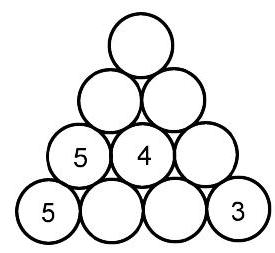
\includegraphics[max width=\textwidth, center]{2024_11_21_67b4ce0009b19a2ea4b2g-1}

\section*{ZADANIE 3.}
Bartek, Maciek i Tomek łowili ryby. Zapytani o to, ile ryb złowili, odpowiedzieli:

\begin{itemize}
  \item Bartek złowił 22 ryby, Maciek 21;
  \item Tomek złowił 19 ryb, a Bartek 21;
  \item Tomek złowił 21 ryb, Maciek 18.
\end{itemize}

Wiadomo, że w każdej odpowiedzi tylko jedna część jest prawdziwa oraz żadni dwaj nie złowili tej samej ilości ryb. Ile ryb złowił każdy chłopiec?

\section*{ZADANIE 4.}
Z prostokąta \(A B C D\) o obwodzie 30 cm wycięto trójkąt równoboczny \(A O D\) o obwodzie 15 cm . Oblicz obwód figury \(A B C D O\).\\
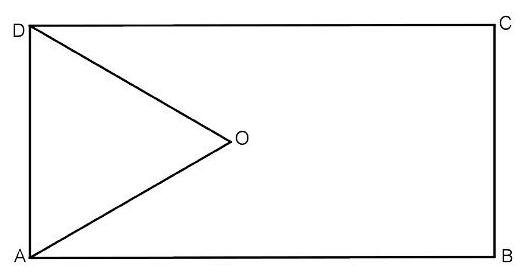
\includegraphics[max width=\textwidth, center]{2024_11_21_67b4ce0009b19a2ea4b2g-1(1)}

\section*{ZADANIE 5.}
Na ławce siedzi Ania, jej mama, babcia i dziadek. Babcia siedzi obok Ani, ale nie siedzi obok dziadka. Dziadek nie siedzi obok mamy Ani. Kto siedzi obok mamy?


\end{document}